\documentclass[border=10pt]{standalone}
\usepackage{tikz}
\usetikzlibrary{arrows.meta}

\begin{document}
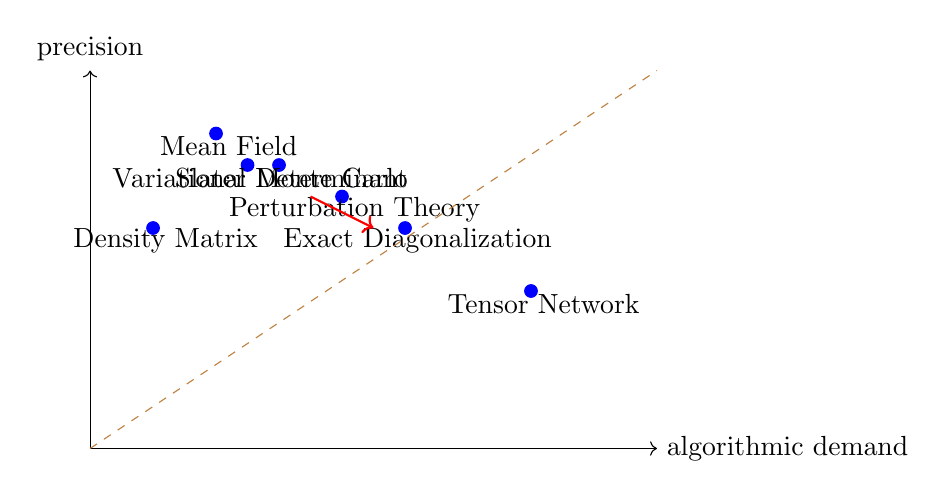
\begin{tikzpicture}[scale=0.8]
    % Axes
    \draw[->] (0,0) -- (9,0) node[right] {algorithmic demand};
    \draw[->] (0,0) -- (0,6) node[above] {precision};

    % Points
    \foreach \x/\y/\label in {
        2/5/{Mean Field},
        3/4.5/{Slater Determinant},
        4/4/{Perturbation Theory},
        5/3.5/{Exact Diagonalization},
        7/2.5/{Tensor Network},
        1/3.5/{Density Matrix},
        2.5/4.5/{Variational Monte Carlo}
    }{
        \filldraw[blue] (\x,\y) circle (0.1);
        \node at (\x+0.2,\y-0.2) {\label};
    }

    % Dashed line
    \draw[dashed, brown] (0,0) -- (9,6);

    % Arrow for Slater Determinant
    \draw[red, thick, ->] (3.5,4) -- (4.5,3.5);
\end{tikzpicture}
\end{document}